\counterwithin{equation}{chapter} % Use chapter as driver for the resetting


\textbf{\LARGE osn 24. Линейные методы в машинном обучении: линейная и гребневая регрессии, метод опорных векторов. Регуляризация в линейных методах. }  \\

Пусть есть множество объектов $\mathbb{X}$, а мы хоти каждому объекту сопоставить какое-то значение.
Числа, которым мы хотим сопоставить объекты из нашего множества иногда называют таргетами.
Таким образом, задачи классификации и регрессии можно сформулировать как поиск отображения из множества объектов $\mathbb{X}$ в множество возможных таргетов.

Математически задачи можно описать так:
\begin{itemize}
    \item \textbf{классификация}: $\mathbb{X} \xrightarrow{}0,1,...,K,$ где $0,..,K$-номера классов
    \item \textbf{регрессия}:  $\mathbb{X} \xrightarrow{} \mathbb{R}$
\end{itemize}
Очевидно, что просто сопоставить какие-то объекты каким-то числам — дело довольно бессмысленное. Нужен критерий качества. Мы бы хотели найти такое отображение, которое лучше всего приближает истинное соответствие между объектами и таргетами. Возможных отображений может быть много, но мы будем искать решение в семействе линейных функций вида 
\begin{equation*}
    y = \omega_1x_1+...+\omega_Dx_D+\omega_0,
\end{equation*}
где $y$ – целевая переменная (\textbf{таргет}), $(x_1,...,x_D)$– вектор, соответствующий объекту выборки (\textbf{вектор признаков}), а $\omega_1,...,\omega_D,\omega_0$ – параметры модели. Вектор $\omega=(\omega_1,...,\omega_D)$ часто называют \textbf{вектором весов}, так как на предсказание модели можно смотреть как на взвешенную сумму признаков объекта, а число $\omega_0$– свободным коэффициентом, или \textbf{сдвигом} (bias). Более компактно линейную модель можно записать в виде
\begin{equation*}
    y = \langle{x, \omega}\rangle+\omega_0,
\end{equation*}
Таким образом, мы ищем не какое-то абстрактное отображение, а конкретный вектор $(\omega_0,\omega_1,...,\omega_D) \in \mathbb{R}^{D+1}.$ \\

Разберёмся, как будет работать такая модель в случае, если $D=1$. То есть у наших объектов есть ровно один численный признак, по которому они отличаются. Теперь наша линейная модель будет выглядеть совсем просто: $y=\omega_1x_1+\omega_0$. Для задачи регрессии мы теперь пытаемся приблизить значение $y$ какой-то линейной функцией от переменной $x$. А что будет значить линейность для задачи классификации? Рассмотрим пример с поиском мошеннических транзакций по картам. Допустим, нам известна ровно одна численная переменная — объём транзакции. Для бинарной классификации транзакций на законные и потенциально мошеннические мы будем искать так называемое \textbf{разделяющее правило}: там, где значение функции положительно, мы будем предсказывать один класс, где отрицательно – другой. В нашем примере простейшим правилом будет какое-то пороговое значение объёма транзакций, после которого есть смысл пометить транзакцию как подозрительную. В случае более высоких размерностей вместо прямой будет гиперплоскость с аналогичным смыслом.  Если мы подозреваем, что целевая переменная $y$ не выражается через $x_1, x_2$ как линейная функция, а зависит ещё от логарифма $x_1$ и ещё как-нибудь от того, разные ли знаки у признаков, то мы можем ввести дополнительные слагаемые в нашу линейную зависимость, просто объявим эти слагаемые новыми переменными и добавив перед ними соответствующие регрессионные коэффициенты
\begin{equation*}
    y \approx \omega_1x_1+\omega_2x_2+\omega_3\log{x_1}+\omega_4sgn(x_1x_2)+\omega_0,
\end{equation*}
и в итоге из двумерной нелинейной задачи мы получили четырёхмерную линейную регрессию.
\begin{center}
    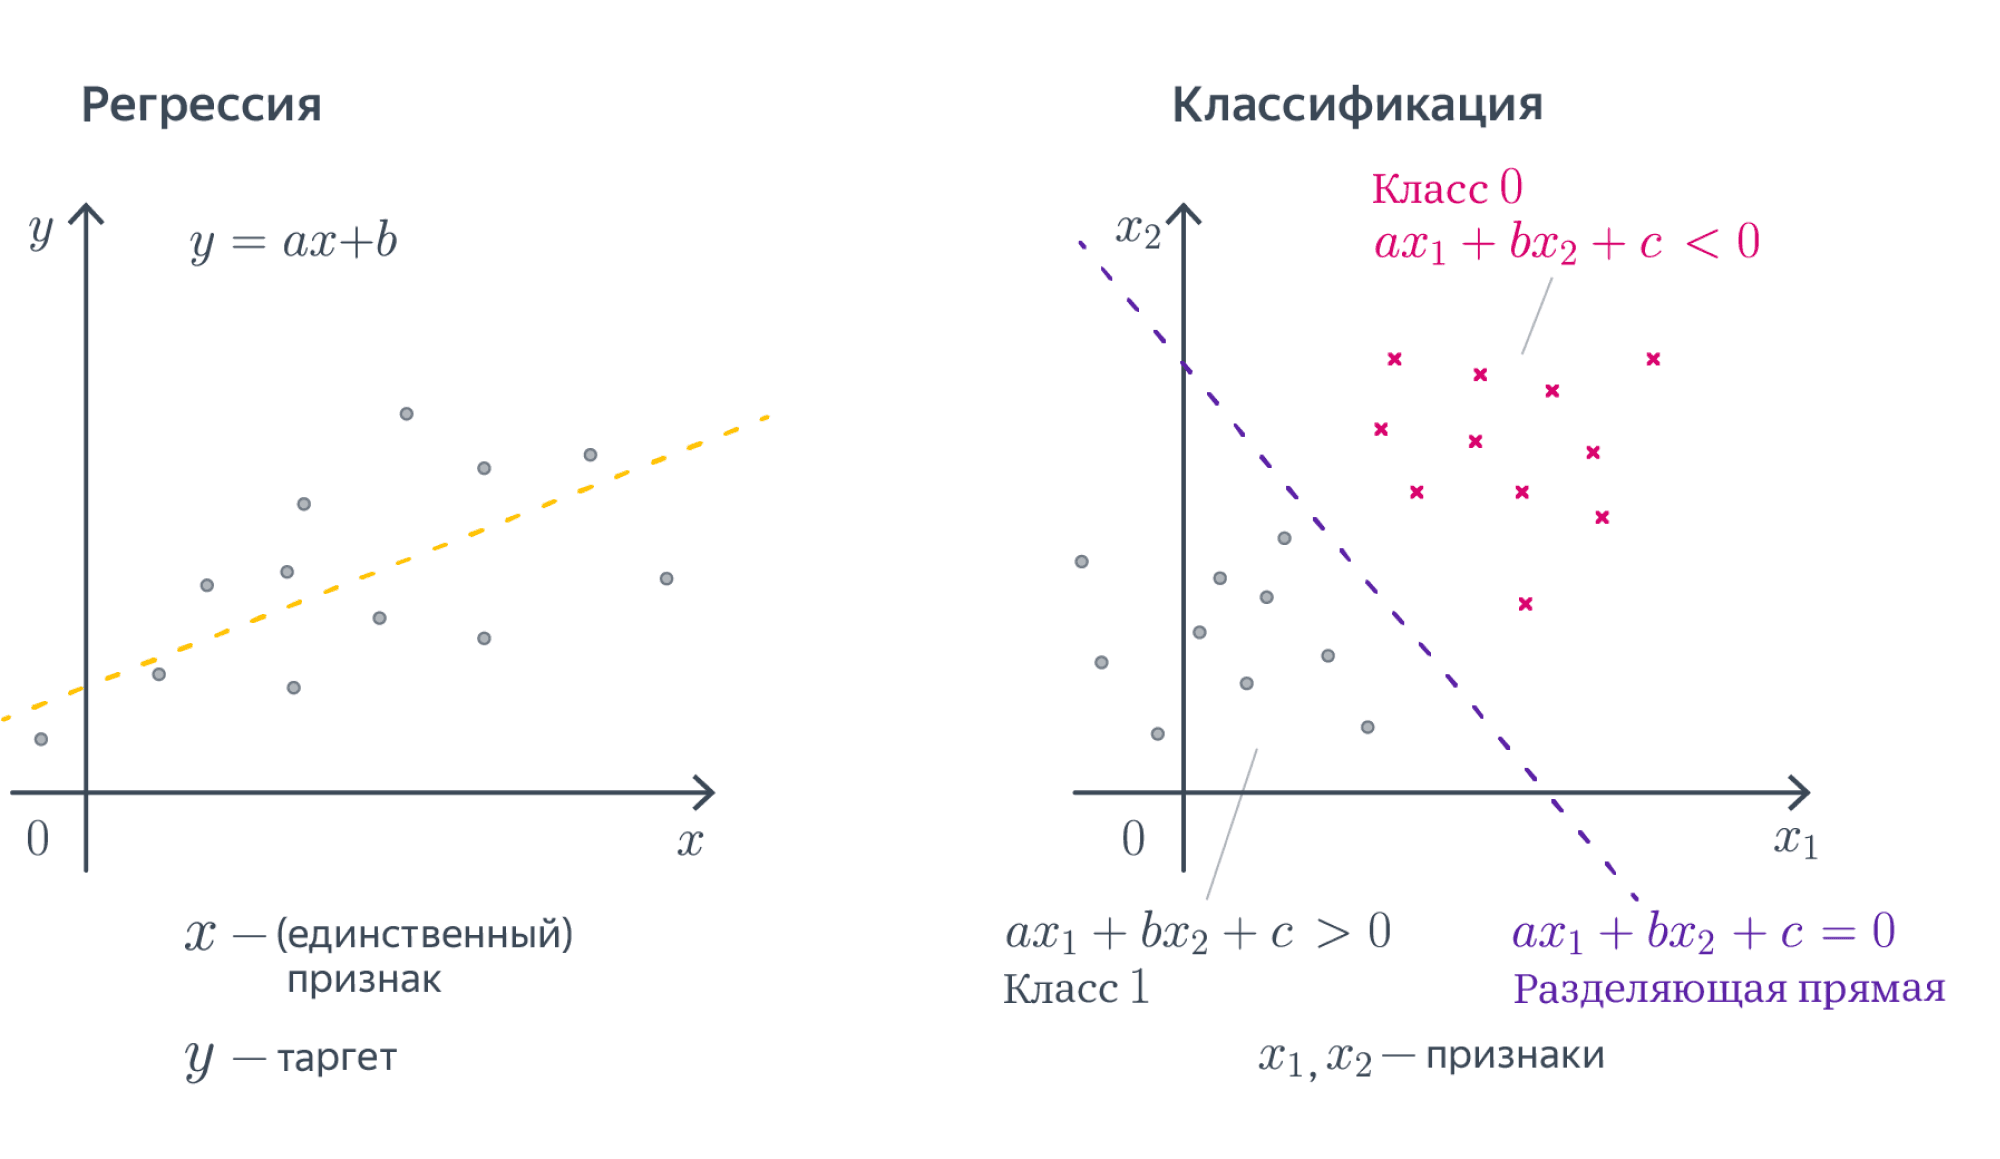
\includegraphics[height=6cm]{pics/t_osn24_linear_models.png}
\end{center}

Если один из признаков является категориальным, то есть принимает значения из (обычно конечного числа) значений, то самый простой способ – использовать \textbf{one-hot кодирование}. Пусть исходный признак мог принимать $M$ значений $c_1,...,c_M$. Давайте заменим категориальный признак на $M$ признаков, которые принимают значения 0 и 1: i-ый будет отвечать на вопрос «принимает ли признак значение?». Иными словами, вместо ячейки со значением $c_i$ у объекта появляется строка нулей и единиц, в которой единица стоит только на i-ом месте. Можно было бы на этом остановиться, но добавленные признаки обладают одним неприятным свойством: в каждом из них ровно одна единица, так что сумма соответствующих столбцов равна столбцу из единиц. Но у нас есть вес $\omega_0$, который соответствует константному признаку, то есть мы получили линейную зависимость признаков. Следовательно, \textbf{от одного из новых признаков можно избавиться}, не меняя модель. Это стоит сделать, потому что наличие «лишних» признаков ведёт к переобучению или вовсе ломает модель.\\
\\
{\large \textbf{Метод наименьших квадратов (МНК)}} \\
Пусть у нас задан датасет $(X, y)$, где 
$y=(y_i)_{i=1}^N \in \mathbb{R}^{N}$ – вектор значений целевой переменной, а $X=(x_i)_{i=1}^N \in \mathbb{R}^{N+D}, x_i \in \mathbb{R}^{N}$– матрица объекты-признаки, в которой 
$i$-я строка – это вектор признаков 
$i$-го объекта выборки. Мы хотим моделировать зависимость $y_i$ от $x_i$ как линейную функцию со свободным членом. Общий вид такой функции из $\mathbb{R}^D$ в $\mathbb{R}$ выглядит следующим образом:

\begin{equation*}
    f_{\omega}(x_i)=\langle\omega,x_i\rangle+\omega_0
\end{equation*}

Свободный член $\omega_0$ часто опускают, потому что такого же результата можно добиться, добавив ко всем $x_i$ признак, тождественно равный единице. Будем считать, что это уже сделано и зависимость имеет вид просто $f_\omega(x_i)=\langle\omega,x_i\rangle$. \\
\textbf{Сведение к задаче оптимизации} \\
Мы хотим, чтобы на нашем датасете (то есть на парах $(x_i, y_i)$ из обучающей выборки) функция $f_\omega$ как можно лучше приближала нашу зависимость.
\begin{center}
    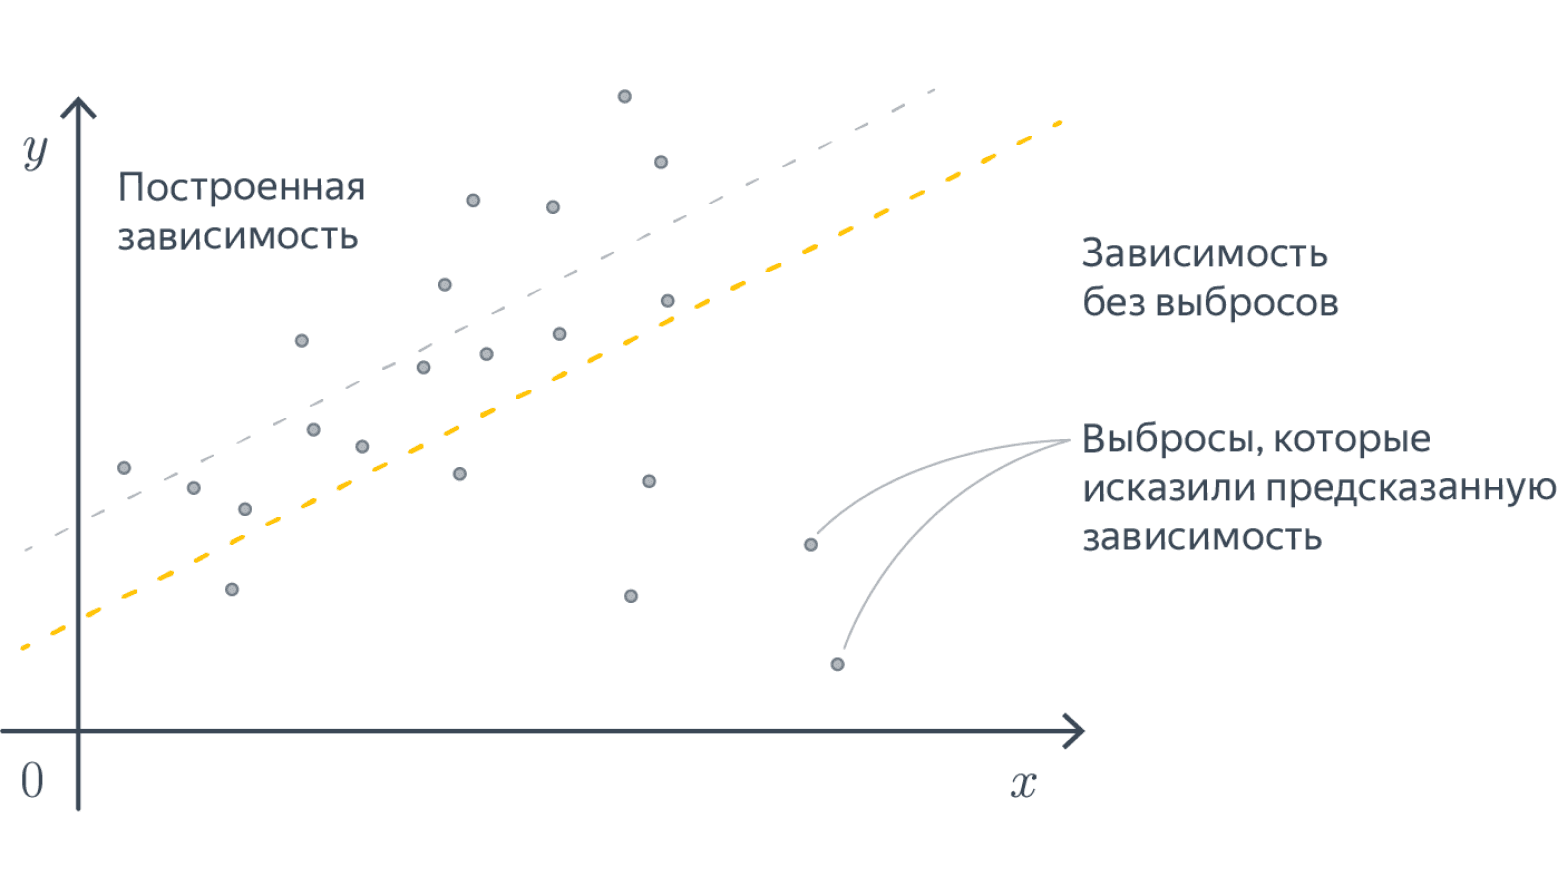
\includegraphics[height=4cm]{pics/t_osn24_2.png}
\end{center}
Мы должны научиться измерять качество модели и минимизировать её ошибку, как-то меняя обучаемые параметры. В нашем примере обучаемые параметры — это веса $\omega$. Функция, оценивающая то, как часто модель ошибается, называется функцией потерь, функционалом качества или лоссом. Важно, чтобы её было легко оптимизировать: скажем, гладкая функция потерь – это хорошо, а кусочно постоянная – плохо.

Для нашей текущей задачи нам нужно взять вектор $y$ и вектор предсказаний модели и как-то сравнить, насколько они похожи.Расстояние между ними вполне может быть функцией потерь. Положительная непрерывная функция от этого расстояния тоже подойдёт в качестве функции потерь. Возьмем в качестве лосса квадрат $L_2$-нормы вектора разницы предсказаний модели и $y$. $L-2$-норма разницы – это евклидово расстояние между вектором таргетов и вектором ответов модели, то есть мы их приближаем в смысле самого простого и понятного «расстояния».
Так вот, наша функция потерь выглядит так:
\begin{equation*}
    L(f,X,y)=\frac{1}{N}|y-f(X)|_2^2=\frac{1}{N}||y-X\omega||_2^2 =\frac{1}{N}\sum_{i=1}^{N} (y_i-\langle x_i,\omega\rangle)^2
\end{equation*}
Такая функция потерь называется \textbf{Mean Squared Error, MSE или среднеквадратическим отклонением}. \\
Для того чтобы найти лучшую модель, этот функционал нам надо минимизировать по $\omega$: $|y-X\omega|_2^2 \xrightarrow{} \min_{\omega}$

Эту задачу можно решить как аналитически, так и приближенно (например градиентным спуском).
Для точного решения необходимо обратить матрицу $X^TX$, а она может быть вырождена или плохо обусловлена из-за приближенной линейной зависимости признаков. \\

\textbf{Регуляризация} \\
Всегда ли решение задачи регрессии единственно? Вообще говоря, нет. Так, если в выборке два признака будут линейно зависимы (и следовательно, ранг матрицы будет меньше $D$), то гарантировано найдётся такой вектор весов $\nu$, что $\langle\nu,x_i\rangle=0  
 $ $\forall x_i$. В этом случае, если какой-то $\omega$ является решением оптимизационной задачи, то и $\omega+\alpha\nu$ тоже является решением для любого $\alpha$. То есть решение не только не обязано быть уникальным, так ещё может быть сколь угодно большим по модулю. Это создаёт вычислительные трудности. Малые погрешности признаков сильно возрастают при предсказании ответа, а в градиентном спуске накапливается погрешность из-за операций со слишком большими числами. В жизни редко бывает так, что признаки строго линейно зависимы, а вот быть приближённо линейно зависимыми они вполне могут быть. Такая ситуация называется \textbf{мультиколлинеарностью}. В этом случае у нас, всё равно, возникают проблемы, близкие к описанным выше. \\
Важно ещё отметить, что в случае, когда несколько признаков линейно зависимы, веса $\omega_i$ при них теряют физический смысл. Может даже оказаться, что вес признака, с ростом которого таргет, казалось бы, должен увеличиваться, станет отрицательным. Это делает модель не только неточной, но и принципиально не интерпретируемой. Вообще, неадекватность знаков или величины весов – хорошее указание на мультиколлинеарность. \\

Для того, чтобы справиться с этой проблемой, задачу обычно \textbf{регуляризуют}, то есть добавляют к ней дополнительное ограничение на вектор весов. Это ограничение можно, как и исходный лосс, задавать по-разному, но, как правило, ничего сложнее, чем $L_1$ (или \textbf{Лассо регуляризация}) и $L_2$ (или \textbf{гребневая регрессия}) -нормы, не требуется. \\
Вместо исходной задачи теперь предлагается решить такую:
\begin{equation*}
    \min_{\omega}L(f, X, y) = \min_{\omega}(|X\omega-y|_2^2+\lambda|w|_k^k)
\end{equation*}
$\lambda$ - это очередной параметр, a $|\omega|_k^k$ - это один из двух вариантов:
\begin{equation*}
    |\omega|_2^2=\omega_1^2+...+\omega_D^2
\end{equation*}
или
\begin{equation*}
    |\omega|_1^1=|\omega_1|+...+|\omega_D|
\end{equation*}
Добавка $\lambda|w|_k^k$ называется \textbf{регуляризационным членом} или \textbf{регуляризатором}, а число $\lambda$ – \textbf{коэффициентом регуляризации}.

Линейная классификация
Теперь давайте поговорим про задачу классификации. Для начала будем говорить про бинарную классификацию на два класса. Её легко обобщить до задачи классификации на $K$ классов. Пусть теперь таргеты $y$ кодируют принадлежность к положительному или отрицательному классу, то есть принадлежность множеству -1 и 1, а $x$– по-прежнему векторы из $\mathbb{R}^D$. Мы хотим обучить линейную модель так, чтобы плоскость, которую она задаёт, как можно лучше отделяла объекты одного класса от другого.
\begin{center}
    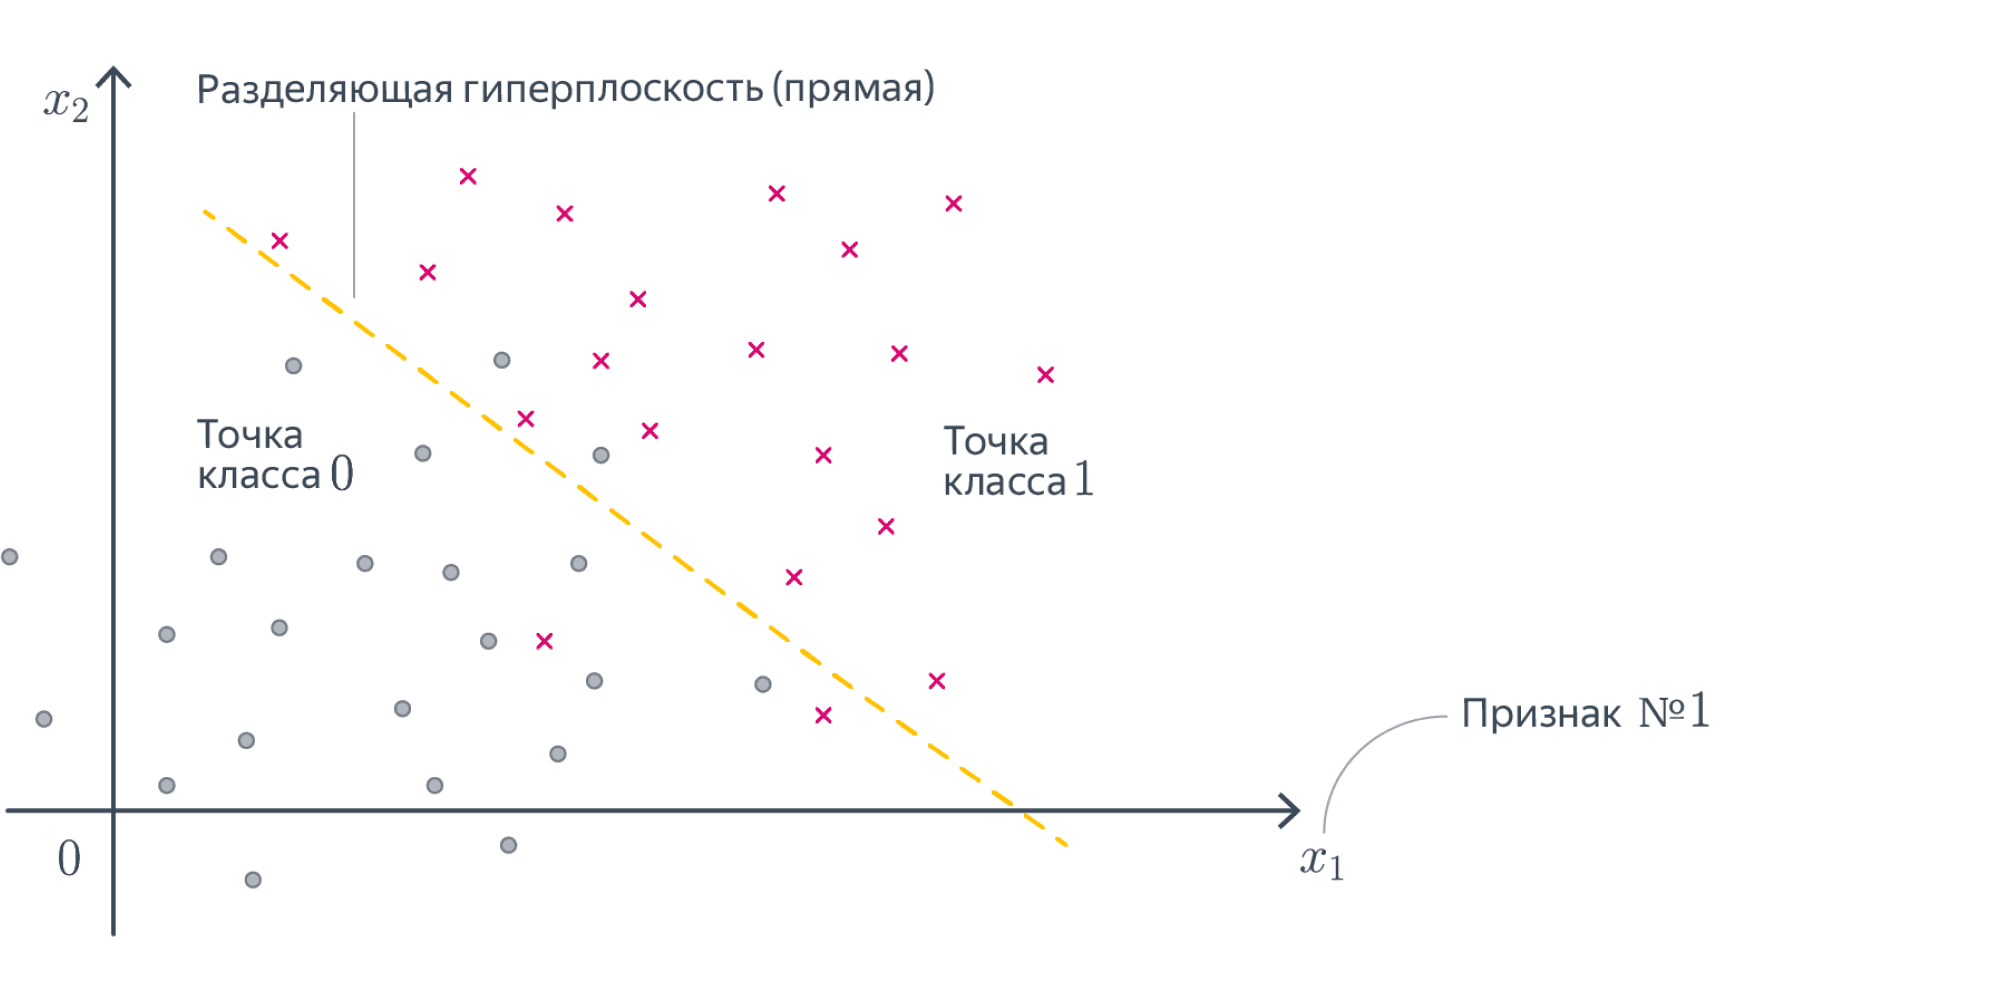
\includegraphics[height=4cm]{pics/t_osn24_3.png}
\end{center}
В идеальной ситуации найдётся плоскость, которая разделит классы: положительный окажется с одной стороны от неё, а отрицательный с другой. Выборка, для которой это возможно, называется линейно разделимой. \\
Итоговое предсказание можно будет вычислить по формуле $y = sign\langle\omega,x\rangle$

Сконструируем теперь функционал ошибки. Мы хотим минимизировать число ошибок классификатора, то есть $$\sum_i \mathbb{I}[y_i \neq sign \langle w, x_i\rangle]\longrightarrow \min_w$$ 

Домножим обе части на $y_i$ и немного упростим $$\sum_i \mathbb{I}[y_i \langle w, x_i\rangle < 0]\longrightarrow \min_w$$ Величина $M = y_i \langle w, x_i\rangle$ называется \textbf{отступом} (margin) классификатора. Такая функция потерь называется \textbf{misclassification loss}. Легко видеть, что отступ положителен, когда $sign(y_i) = sign(\langle w, x_i\rangle)$, то есть класс угадан верно; при этом чем больше отступ, тем больше расстояние от $x_i$ до разделяющей гиперплоскости, то есть «уверенность классификатора»; отступ отрицателен, когда $sign(y_i) \ne sign(\langle w, x_i\rangle)$, то есть класс угадан неверно; при этом чем больше по модулю отступ, тем более сокрушительно ошибается классификатор. От каждого из отступов мы вычисляем функцию $$F(M) = \mathbb{I}[M < 0] = \begin{cases}1,\ M < 0,\\ 0,\ M\geqslant 0\end{cases}$$ Она кусочно-постоянная, и из-за этого всю сумму невозможно оптимизировать градиентными методами: ведь её производная равна нулю во всех точках, где она существует. Но мы можем мажорировать её какой-нибудь более гладкой функцией, и тогда задачу можно будет решить.  \\

\textbf{Hinge loss, SVM} \\
Возникает логичное желание не только найти разделяющую прямую, но и постараться провести её на одинаковом удалении от обоих классов, то есть максимизировать минимальный отступ:
\begin{center}
    \centering
    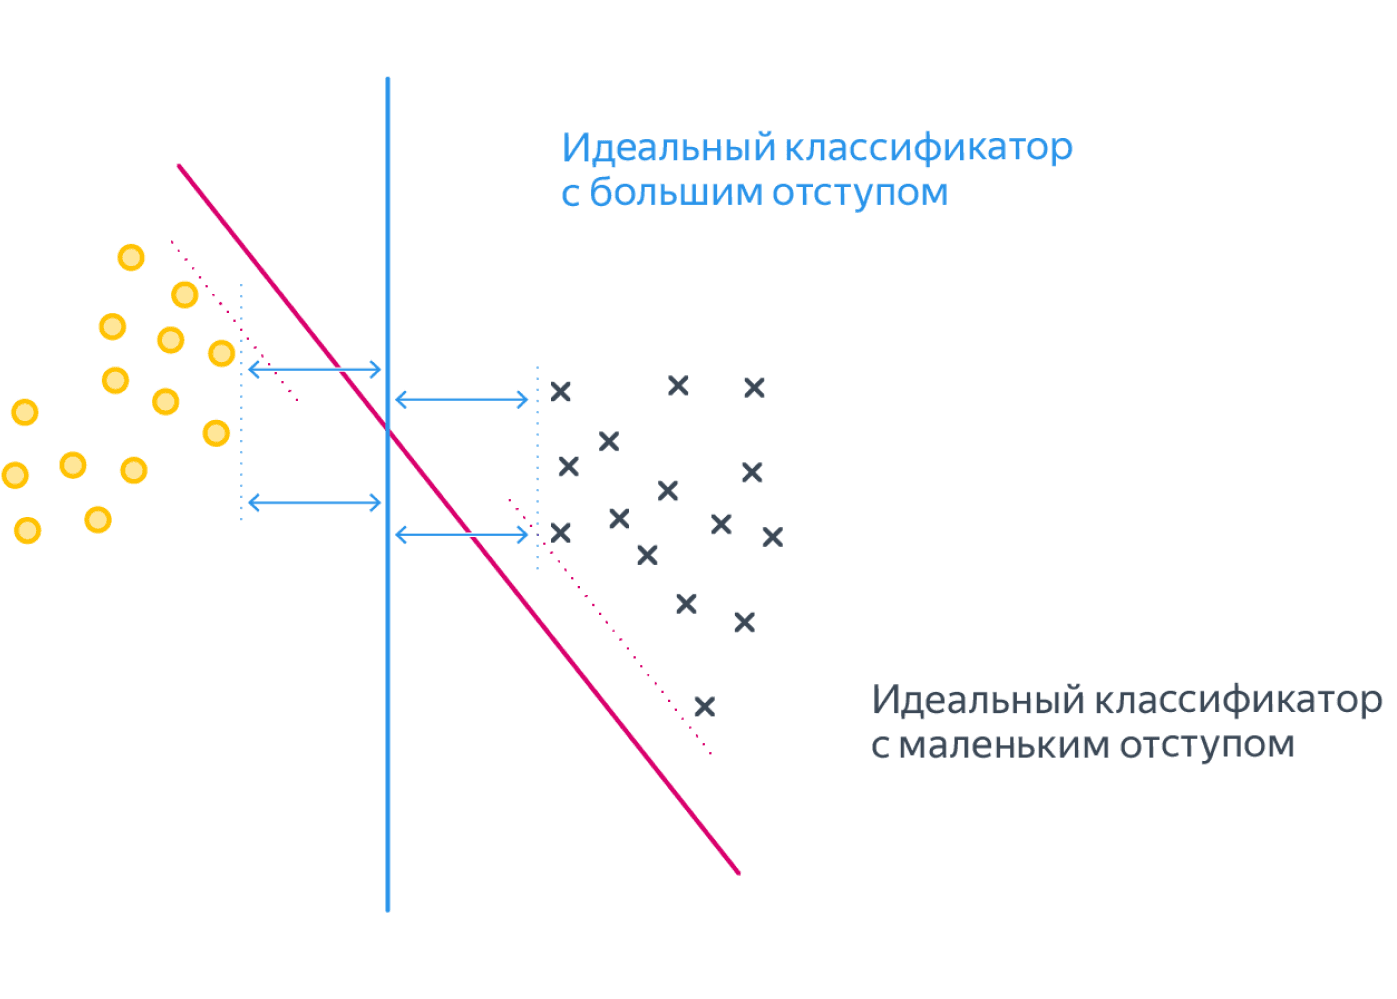
\includegraphics[height=4cm]{pics/t_osn24_4.png}
\end{center}
Это можно сделать, слегка поменяв функцию ошибки, а именно положив её равной:
$$F(M) = \max(0, 1-M)$$
$$L(w, x, y) = \lambda||w||^2_2 + \sum_i \max(0, 1-y_i \langle w, x_i\rangle)$$
$$\nabla_w L(w, x, y) = 2 \lambda w + \sum_i
        \begin{cases} 
             0,      & \quad      1 - y_i \langle w, x_i \rangle \leq 0 \\ 
            - y_i x_i, & \quad   1 - y_i \langle w, x_i \rangle > 0
        \end{cases}$$ 
Почему же добавленная единичка приводит к желаемому результату? \\ Интуитивно это можно объяснить так: объекты, которые проклассифицированы правильно, но не очень "уверенно" (то есть $0 \leq y_i \langle w, x_i\rangle < 1$), продолжают вносить свой вклад в градиент и пытаются "отодвинуть" от себя разделяющую плоскость как можно дальше. \\
К данному выводу можно прийти и чуть более строго; для этого надо совершенно по-другому взглянуть на выражение, которое мы минимизируем. Поможет вот эта картинка:
\begin{center}
    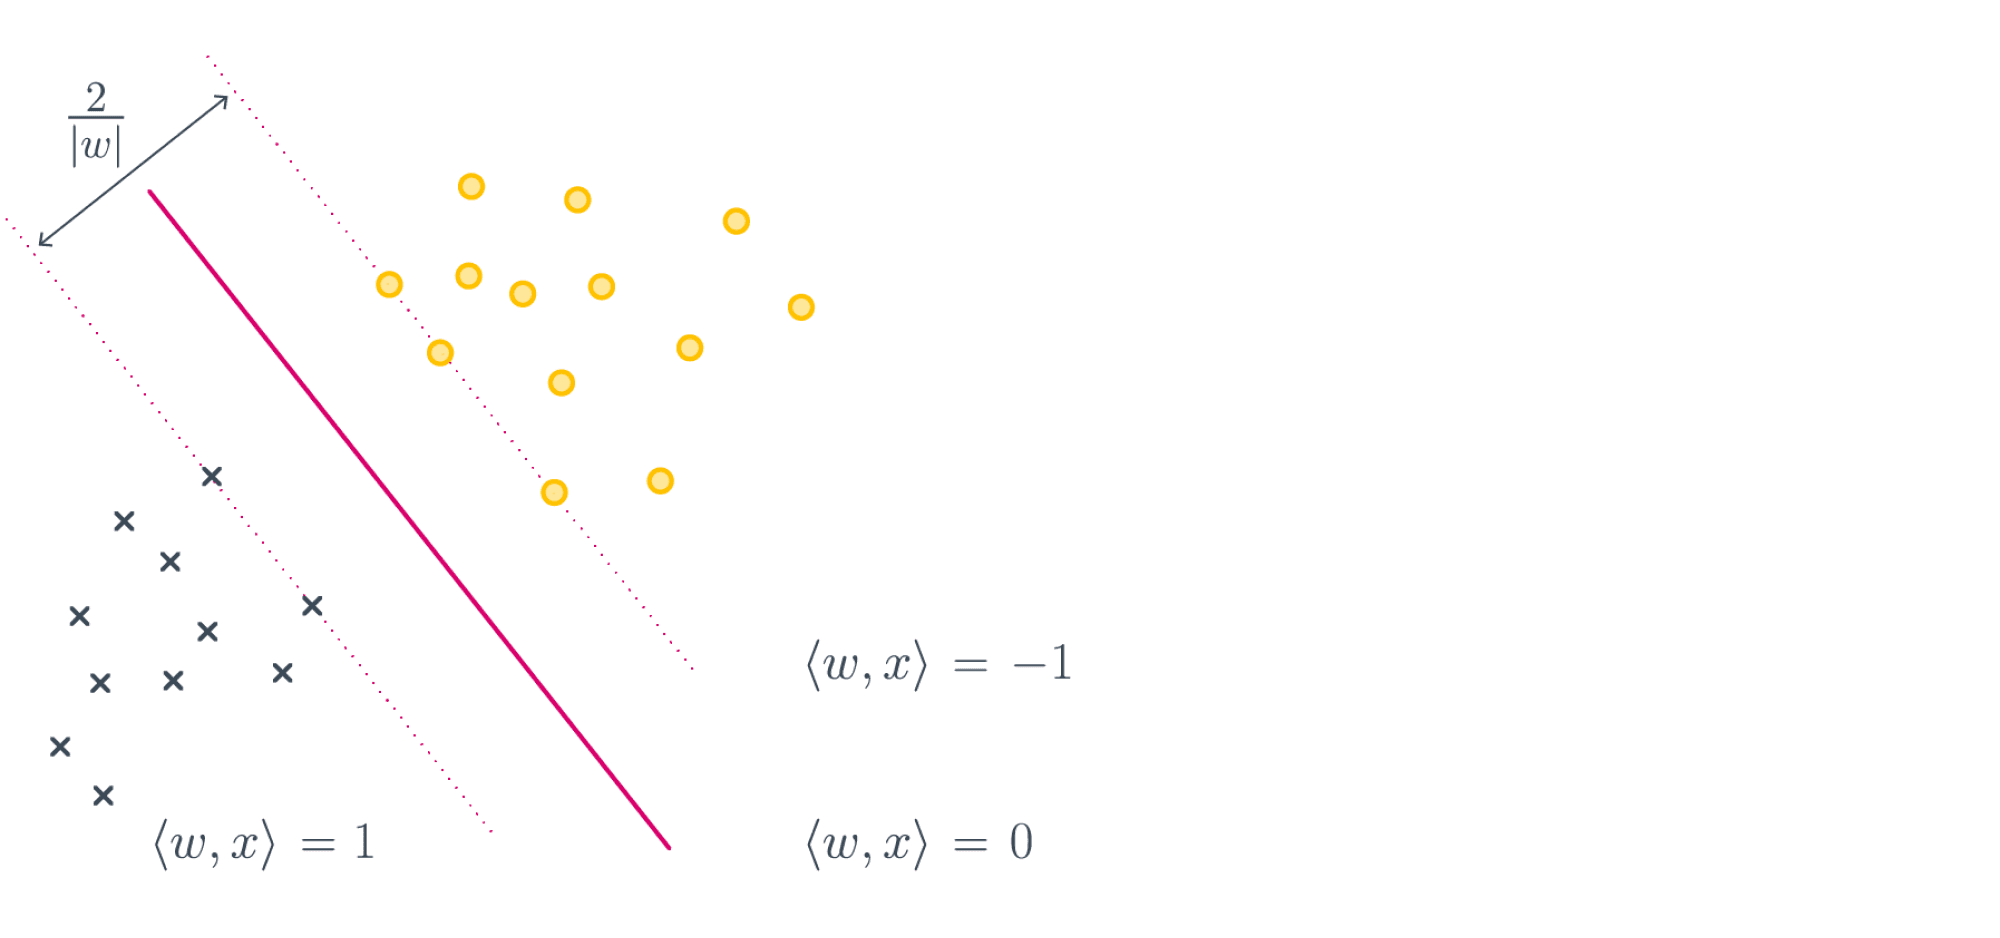
\includegraphics[height=4cm]{pics/t_osn24_5.png}
\end{center}
Если мы максимизируем минимальный отступ, то надо максимизировать $\frac{2}{|w|_2}$, то есть ширину полосы при условии того, что большинство объектов лежат с правильной стороны, что эквивалентно решению нашей исходной задачи:
$$\lambda|w|^2_2 + \sum_i \max(0, 1-y_i \langle w, x_i\rangle) \longrightarrow\min\limits_{w}$$
Отметим, что первое слагаемое у нас обратно пропорционально ширине полосы, но мы и максимизацию заменили на минимизацию, так что тут всё в порядке. Второе слагаемое – это штраф за то, что некоторые объекты неправильно расположены относительно разделительной полосы, так как классы могут быть линейно неразделимы. \\
Итоговое положение плоскости задаётся всего несколькими обучающими примерами. Это ближайшие к плоскости правильно классифицированные объекты, которые называют \textbf{опорными векторами} или \textbf{support vectors}. Весь метод, соответственно, зовётся методом \textbf{опорных векторов}, или \textbf{support vector machine}, или сокращённо \textbf{SVM}. 

% -------- source --------
\bigbreak
[\cite{t_osn24_svm_mlbook}]